\chapter{Data set}\label{chap:dataset}
Recommender systems rely on data for their development, training and evaluation. It is therefore important to properly assess potential data sets in terms of their strengths and shortcomings---especially with regards to the task at hand. In citation recommendation, the goal is to identify papers relevant to a user input. Because of the large amount of available research, this means a recommender has to be able to find relevant publications in a large set of possible candidates in order to be considered fit for the task. As a comsequence, evaluation results are likely to be more meaningful when a large data set is used. Apart from the size, the quality of data is also crucial. For local citation recommendation this means that a clean citation context, precise position of citaiton markers and valid citation information are desirable. With these criteria in mind we assessed existing data sets, leading us to the conclusion that---for the relatively new task of local citation recommendation---it would be worth the effort to create a new data set.

The following sections describe the details of our assessment as well as the creation process and evaluation of our new data set.

\section{Existing data sets}

\begin{table}
\centering
    \caption{Overview of existing data sets.}
    \label{tab:datasets}
\begin{center}
    % \caption{Overview of existing data sets.}
    % \label{tab:existing-data-sets}
    \begin{tabular}{lllll}
    \toprule
    Data set & \#Papers & Cit. context & Disciplines & Ref. IDs \\
    \midrule
    CiteSeerX~\cite{Caragea2014} / RefSeer~\cite{Huang2014} & 5M & 400 chars & (unrestricted) & internal \\
    PubMed Central OAS\footnote{\url{https://www.ncbi.nlm.nih.gov/pmc/tools/openftlist/}} & 2.3M & extractable & Biomed./Life Sci. & mixed \\
    arXiv CS~\cite{Faerber2018} &  90K & 1 sentence & CS & DBLP \\
    Scholarly v2\footnote{\url{http://www.comp.nus.edu.sg/~sugiyama/SchPaperRecData.html}}  & 100K & extractable & CS & no \\
    ACL-ARC  & 11K & extractable & CS/Comp. Ling. & no \\ % \cite{Bird2008ACLARC}
    ACL-AAN  & 18K & extractable & CS/Comp. Ling. & no  \\ % \cite{Radev2013}
    \bottomrule
    \end{tabular}
\end{center}
\end{table}

Table~\ref{tab:datasets} gives an overview of relevant existing data sets. While various recommendation domains have established quasi standard data sets, this is not yet the case in citation recommendation. CiteSeerX is currently the most used in the field~\cite{Beel2016}. It is comparatively large, but many approaches only use subsets and generate them with varying filtering criteria. Furthermore, there are several quality issues. The main problems are inaccurate citaion information, noisy citation contexts and cut off words at the borders of citation contexts.

The PubMed Central Open Access Subset is another large data set that has been used for citation based tasks~\cite{Duma2016,Gipp2015,Galke2018,Bhagavatula2018}. Contained publications are already processed and available in XML format. While the data set overall is comparatively clean, heterogeneous annotation of citations within the text and mixed usage of global reference identifiers (PubMed, MEDLINE, DOI, ...) make it difficult to retrieve high quality citation interlinkings of documents from the data set\footnote{To be more precise, the heterogeneity makes the usage of the data set \emph{as is} problematic. Resolving references retrospectively would be an option but comparatively challenging in the case of PubMed because of the frequent usage of special notation in publication titles; see also: \texttt{\url{http://www.sciplore.org/files/citrec/CITREC_Parser_Documentation.pdf}}}~\cite{Gipp2015}.

%MAG\cite{Sinha2015} (use/analysis: \cite{Herrmannova2016,Paszcza2016,Hug2017})

\section{Data set creation}
arXiv operates since 1991\cite{Ginsparg1994}

system to automatically extract citation interlinks from arXiv sources by parsing LaTeX files as early as 1998\cite{Nanba1998}

survey paper on extraction of meta data (author, year, ...) and classification of sentences (method, goal, ...) from publications\cite{Nasar2018}

evaluation of reference string parsers\cite{Tkaczyk2018}, a dataset for reference string parsing\cite{Anzaroot2013}

\section{Data set evaluation}
Scientific publications are usually distributed in formats targeted at human consumption (e.g. PDF) or, in cases like arXiv.org, also as source files \emph{for} the aforementioned (e.g. LaTeX sources for generating a PDF). Citation recommendation, in contrast, requires automated processing of publications' textual contents as well as documents' interlinking through citations. The creation of a data set for citation recommendation therefore encompasses two main steps: extraction of plain text and resolution of references. In the following we will describe how we approached these two steps using arXiv.org publication sources and the Microsoft Academic Graph (MAG)\cite{Sinha2015}.
\subsection{arXiv.org sources and the MAG}
The following two resources are the basis of the data set creation process.

\paragraph{arXiv.org} hosts over 1.4 million submissions from August 1991 onward\footnote{https://arxiv.org/stats/monthly\_submissions}. They are available not only as PDF, but (in most cases) also as LaTeX source files. The discipline most prominently represented is physics, followed by mathematics, with computer science seeing a continued increase in percentage of submissions ranking third. The availability of LaTeX sources makes arXiv.org submissions particularly well suited for extracting plain text and accurate citation information.
\paragraph{Microsoft Academic Graph} is a very large\footnote{At the time of writing the MAG contains data on over 200 million publications.}, automatically generated data set on publications, related entities (authors, venues, etc.) and their interconnections through citation. While citation contexts are available, full text is not. The size of the MAG makes it a good target for matching reference items against it. Especially given that arXiv.org spans several fields of study.
\subsection{Pipeline overview}
To create the data set we start out with arXiv sources. From these we generate, per publication, a plain text file with the document's textual contents and a set of database entries reflecting the document's reference section\footnote{Association between reference items and citations in the text are preserved by placing citation markers in the text.}. In a second step we then iterate through all reference items in the database and match them against paper metadata records in the MAG (See figure \ref{fig:datagen}). The result of this process are MAG paper records associated with one or more reference items, who in turn are associated with citation contexts in the plain text files. In other words, we end up with descriptions of cited documents, consisting of the sections of citing documents aforementioned are referenced in.


\begin{figure}[t]
\begin{centering}
    \subfloat[subfloat]
    {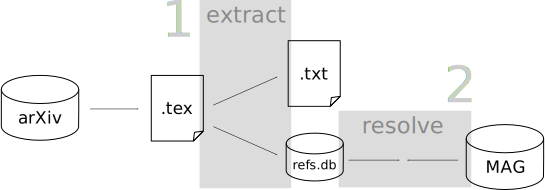
\includegraphics[scale=0.2]{figures/dataset/data_set_generation_schema.pdf}}
    % \subfloat[Some cool related graphic]
    % {\includegraphics[scale=0.4]{figures/experiments/microcontroller.png}}
    \caption[Schematic representation of the data set generation process.]{Schematic representation of the data set generation process.}
  \label{fig:datagen}
\end{centering}
\end{figure}

\subsection{LaTeX parsing}
LaTeX code, albeit structured and guided by rules, is written by humans and offers many possibilities and freedoms, which makes parsing it a non trivial task. Moreover, the generation of a large data set necessitates parsing large quantities of LaTeX sources in a limited amount of time. This means fault tolerance, quality of output and speed are three goals for LaTeX parsing. In the following we will describe the tools considered for this task, the challenges we faced in general and with regard to arXiv sources in particular and the resulting approach.
\subsubsection{Tools}
We considered several tools for direct conversion to plain text or to intermediate formats. Table \ref{tbl:tools} gives an overview.

\begin{table}
\centering
  \caption{Comparison of tools for parsing \LaTeX{}.}
  \label{tbl:tools}
\begin{tabular}{llll}
\toprule
    Tool & Output & Robust & Usable w/o modification \\
   \midrule
    plastex\footnote{\url{https://github.com/tiarno/plastex}} & DOM & no & yes\\
    TexSoup\footnote{\url{https://github.com/alvinwan/texsoup}} & document tree & no & yes\\
    opendetex\footnote{\url{https://github.com/pkubowicz/opendetex}}/detex\footnote{\url{https://www.freebsd.org/cgi/man.cgi?query=detex}} & plain text & no & yes\\
    GrabCite~\cite{Faerber2018} & plain\hphantom{ }text\hphantom{ }+ resolved ref. & yes & no\\
    LaTeXML\footnote{\url{https://github.com/brucemiller/LaTeXML}} & XML & yes & yes\\
    Tralics\footnote{\url{https://www-sop.inria.fr/marelle/tralics/}} & XML & yes & yes\\
  \bottomrule
\end{tabular}
\end{table}

Based on this evaluation we chose to use Tralics to convert the arXiv sources to XML and from there generate plain text and reference item database records. Compared to LaTeXML the output contained a bit more noise---particularly from LaTeX preambles---but the immense speed gain would allow for the generation of a large data set in a reasonable time frame.

\subsubsection{Challenges}
Challenges faced in getting from arXiv sources to plain text range from the source files themselves, over their LaTeX contents to specifics concerning the parsing tool. For some portion of arXiv submissions, LaTeX sources are straight up not available. This can mean that source files are in a different format (like HTML or TeX) or just a PDF is present. In cases where LaTeX sources are available, these have to be correctly identified (file encodings, unorthodox choices of file extensions etc. can be a challenge here) and then can be parsed. In few cases, where the source consists of a single \texttt{\textbackslash includepdf} command, there can be no sensible output. The majority fortunately is proper LaTeX code. Challenges in such cases include the usage of unusual extra packages not included in the source and convoluted (re-)definition of macros. An illustrating and easy to understand case of this is a paper we noticed, where the author chose to create a new command \emph{for the macro} \texttt{\textbackslash newcommand} which they then used to create new commands for adding items to the reference section of the paper.

\subsubsection{Detailed description}
In a first step we go from the various shapes of sources to a single LaTeX file per arXiv submission. If the source consists of a single file, we determine whether or not it's a LaTeX file. In case of more than one file we search for a main LaTeX file, look if a \texttt{.bbl} file is present\footnote{If so, it has to be the same name as the main LaTeX file: https://arxiv.org/help/submit\_tex\#bibtex} and then flatten the LaTeX project to a single file using latexpand\footnote{https://ctan.org/pkg/latexpand}\footnote{We also tested flatex (https://ctan.org/pkg/flatex) and flap (https://github.com/fchauvel/flap) but got the best results with latexpand.}. To prevent parsing problems later on we then normalize \texttt{\textbackslash cite} and \texttt{\textbackslash bibitem} commands (many papers use variations of these commands defined in e.g. the \texttt{natbib} package).

The second step is to convert each LaTeX source to plain text while keeping track of citation markers and reference items. Using Tralics we generate an XML representation of each LaTeX document and replace formulas, figures, tables and non citation references with replacement tokens. The plain text is then extracted, each reference item is assigend a UUID, its text stored in a database and corresponding citation markers are placed in the plain text.

\subsection{Reference resolution}
A single publication's reference section follows a coherent style, many publications can follow many different bibliography styles though. Furthermore, the amount of information included in a reference item is variable and can range from the inclusion of unique identifiers like a DOI up to the omission of the cited work's title. This makes the automated identification of cited documents based on reference items a challenging and still unsolved task\cite{Nasar2018}.

Given it is, by itself, the most distinctive part of a publication, we base our reference resolution on the title of the cited work and use other pieces of information (e.g. authors' names) only in secondary steps. In the following we will describe the challenges we faced, matching arXiv.org submissions' reference items against MAG paper records and how we approached the task.
\subsubsection{Challenges}
The reference resolution process depends on three pieces. Both data records (arXiv side and MAG side) and the matching procedure. Considering the arXiv side, reference items can be problematic when they do not contain a title or contain formulas in the title. Citing by only authors, journal name, volume and article number was often observed by us in physics papers. Formulas can become problematic because of inconsistent ways of transcribing them as plain text. One also comes across reference items that are mere comments (and would have probably better been included as footnotes) or ones that refer to non publications. These cases are less problematic because they just fail to match. The most significant challenge on the MAG side is noise. This can either prevent matches or lead to false matches.

The matching procedure ideally has a certain tolerance for minor inconsistencies (abbreviations or typos for example) while remaining accurate. Another requirement, because of the amount of data, is again speed. As every citing document can have many reference items, the number of reference items to process can easily be an order of magnitude higher than the number of citing documents. This circumstance required us to implement the matching procedure in a parallelized fashion which brought its own set of technical challenges.

\subsubsection{Detailed description}
Our reference resolution approach can be broken down in two steps: title identification and matching. For identification of the title we first look for arXiv IDs and DOIs within the reference item. If such an ID is present we obtain the cited work's title from an arXiv metadata dump or via crossref.org\footnote{https://www.crossref.org/} respectively. Otherwise we use Neural ParsCit\cite{Animesh2018} to identify the portion of the item that makes up the title. Because there are cases where the identified range is just slightly off, we identify several title candidates, beginning with the one identified by Neural ParsCit and then varying the range by a few words. For the matching we then normalize the title the same way the MAG's normalized titles are generated. This means replacing everything not matching the regex word character class \texttt{\textbackslash w} with a space, normalizing modified alphabet characters like umlauts (ö$\rightarrow$o) and finally replacing multiple spaces with single ones. The normalized title is matched against all MAG papers. The resulting match candidates are then checked by author names. A candidate is considered good, if at least of of the author's normalized names in the MAG appears in the normalized reference item string. If, after this, still multiple candidates are left, we order them by the citation count given in the MAG and choose the first one. The last step particularly helps to mitigate rouge almost-duplicate entries in the MAG that often have few to no citations.

\section{Key figures}
\subsection{Creation process}
We used an arXiv.org source dump containing all submissions up until the end of 2017 (1,340,770 documents). 100,240 of these were only available in PDF format, leaving 1,240,530 sources. Our pipeline output 1,151,707 (92.8\%) plain text files, 1,018,976 (82.1\%) of which contained citation markers (for the missing 10\% the parsing of \texttt{\textbackslash cite} and \texttt{\textbackslash bibitem} commands most likely failed). The number of reference items identified is 35,053,329, for which 56,077,906 citation markers were placed within the plain text files. This first part of the process took 59 hours to run, unparallalized on a 8 core Intel Core i7-7700 3.60GHz machine with 60 GB of memory.

Of the 35.053.329 reference items, we were able to match 14,046,239 (40.07\%). For 33.14\% of the reference items we could neither find an arXiv ID or DOI, nor was Neural ParsCit able to identify a title. For the remaining 26.79\% a title was identified but could not be matched with the MAG. Of the matched 14 million items' titles, 50.67\% were identified via Neural ParsCit. 29.67\% by DOI and 19.66\% by arXiv ID. Of the identified DOIs 26.8\% were found as is while 73.2\% were heuristically determined\footnote{This was possible because the DOIs of articles in journals of the American Physical Society follow predictable patterns.}. The matching process took 103 hours, run in 10 parallel processes on a 64 core Intel Xeon Gold 6130 @ 2.10GHz machine with 500 GB of memory.

\subsubsection{Quality assessment of matches} To test the quality of our matches we take a random sample of 300 matched reference items and manually check if the correct record in the MAG was identified. For 300 items we note 3 errors, giving us an accuracy estimate of 96\% at the worst, as shown in table \ref{tbl:confvals}.

\begin{table}
  \caption[Confidence intervals for a sample size of 300 with 297 positive results.]{Confidence intervals for a sample size of 300 with 297 positive results as given by Wilson score interval and Jeffreys interval \cite{Brown2001}.}
  \label{tbl:confvals}
  \centering
  \begin{small}
\begin{tabular}{c@{\hspace{0.1in}}c@{\hspace{0.1in}}c@{\hspace{0.1in}}c}
\toprule
    Confidence level & Method & Lower limit & Upper limit \\\noalign{\smallskip}
\midrule
    0.99 & Wilson & 0.9613 & 0.9975 \\\noalign{\smallskip}
    \ & Jeffreys & 0.9666 & 0.9983 \\\noalign{\smallskip}
    \hline\noalign{\smallskip}
    0.95 & Wilson & 0.9710 & 0.9966 \\\noalign{\smallskip}
    \ & Jeffreys & 0.9736 & 0.9972 \\\noalign{\smallskip}
    \bottomrule
\end{tabular} 
\end{small}
\end{table}

The three incorrectly identified references were as follows (MAG IDs in square brackets):
\begin{enumerate}
    \item \emph{''Eddy, J.A.: 1983, The maunder minimum - a reappraisal. Solar Phys. 89, 195. ADS.''}
    \begin{itemize}
        \item matched: [\texttt{2024069573}]\\\emph{''The Maunder Minimum''} (John A. Eddy; 1976)
        \item correct: [\texttt{2080336740}]\\\emph{''The Maunder Minimum: A reappraisal''} (John A. Eddy; 1983)
    \end{itemize}
    \item \emph{''J. Zhu, S. Rosset, T. Hastie, and R. Tibshirani. 1-norm support vector machines. In Advances in Neural Information Processing Systems (NIPS), volume 16, pages 49–56, 2004.''}
    \begin{itemize}
        \item matched: [\texttt{2249237221}]\\\emph{''Support Vector Machines''} (Gareth James, Daniela Witten, Trevor Hastie, Robert Tibshirani; 2013)
        \item correct: [\texttt{2130698119}]\\\emph{''1-norm Support Vector Machines''} (Ji Zhu, Saharon Rosset, Robert Tibshirani, Trevor J. Hastie; 2003)
    \end{itemize}
    \item \emph{''D. T. Limmer and D. Chandler. The putative liquid-liquid transition is a liquid-solid transition in atomistic models of water. The Journal of Chemical Physics, 135(13):134503, 2011.''}
    \begin{itemize}
        \item matched: [\texttt{2599889364}]\\\emph{''The Putative Liquid-Liquid Transition is a Liquid-Solid Transition in Atomistic Models of Water''} (David Chandler, David Limmer; 2013)
        \item correct: [\texttt{1977410206}]\\\emph{''The putative liquid-liquid transition is a liquid-solid transition in atomistic models of water. II''} (David T. Limmer, David Chandler; 2011)
    \end{itemize}
\end{enumerate}
\subsection{Resulting data set}
For the resulting data set we first report the number of cited papers, citing papers, references and citation contexts. Figure \ref{fig:fournumbers} illustrates these four types of numbers in a small toy example for ease of understanding. For our data set we ended up with 2,343,585 cited papers, 926.644 citing papers, 13,303,373 references and 24,558,560 citation contexts. Note that these numbers do not reflect the ones reported for the generation process exactly. This is because references can end up with no associated citation contexts due to parsing problems. Such cases are not counted for the data set.

\begin{figure}
  \centering
    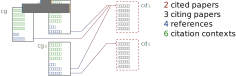
\includegraphics[width=\textwidth]{figures/dataset/four_types_of_numbers_vertsqueeze.pdf}
  \caption[Four types of numbers.]{Four types of numbers. A toy example with citation pairs $cg_1\rightarrow cd_1$, $cg_2\rightarrow cd_1$, $cg_3\rightarrow cd_1$, $cg_3\rightarrow cd_2$ resulting in 2 cited papers, 3 citing papers, 4 references and 6 citation contexts.}
  \label{fig:fournumbers}
\end{figure}

Figure \ref{fig:numcitdoc} shows the number of citing documents for all cited documents. There is one document with close to 10,000 citations, another 3 with more than 5,000 and another 10 with more than 3,000. 1,262,861 (53.89\%) of the documents have at least 2 citations, 547,036 (23.34\%) have at least 5. The mean number of citations is 5.68 (SD 26.82). Figure \ref{fig:numcontref} shows the number of citation context per reference. 8,722,795 (65.57\%) references have only one citation context, the maximum is 278, the mean 1.85 (SD 2.02). This means a cited document is described by on average $1.85 \times 5.68 \approx 10.5$ citation contexts.

\begin{figure}[tb]
  \centering
  \includegraphics[width=\linewidth]{figures/dataset/citing_docs_per_cited_doc.pdf}
  \caption{Number of citing documents per cited document.}
  \label{fig:numcitdoc}
\end{figure}

\begin{figure}[tb]
  \centering
  \includegraphics[width=\linewidth]{figures/dataset/citation_contexts_per_reference.pdf}
  \caption{Number of citation contexts per reference.}
  \label{fig:numcontref}
\end{figure}

Figure \ref{fig:sankey} shows the flow of citations by field of study for all 13.3 million matched reference items. Fields of study with very small numbers of references are combined to \emph{other} for legibility reasons. For the citing document's side, these are economics, electrical engineering and systems science, quantitative biology, quantitative finance and statistics. Combined on the cited document's side are chemistry, biology, engineering, materials science, economics, geology, psychology, medicine, business, geography, sociology, political science, philosophy, environmental science and art. In rare cases\footnote{Exact numbers for the whole MAG are as follows: physics 8,682,931; math 6,701,038; cs 14,225,297; cs+math 2,254; math+phys 1,737; phys+cs 287.} papers in the MAG (cited document's side) can have multiple main fields of study assigned. In such an event we assigned the first one we retrieved from the MAG.

\begin{figure}
  \centering
    \includegraphics[width=\textwidth]{figures/dataset/citation_relation_sankey.pdf}
  \caption[Citation flow by field of study for 13.3 million reference items.]{Citation flow by field of study for 13.3 million reference items. For reference, the number of citing and cited documents per field of study are plotted on the sides.}
  \label{fig:sankey}
\end{figure}

To no surprise, publications in each field are cited the most from within the field itself. Notable is, however, that the incoming citations in mathematics are the most varied (physics and computer science combined make up 38\% of the citations).
